%%%%%%%%%%%%%%%
% EFT Paper
% v.1
% R. Itay & B. Farmer & A. Manfredini
%%%%%%%%%%%%%%%

\RequirePackage{lineno}
\documentclass[twocolumn, showpacs, showkeys, amsmath, amssymb, floatfix]{revtex4} 
\usepackage[colorlinks=true, citecolor=green, filecolor=blue, linkcolor=blue, urlcolor=blue]{hyperref}
\usepackage{color}
\usepackage{graphicx}
\usepackage[perpage]{footmisc}
	
\newcommand \Leff{$\mathcal{L}_{\mathrm{eff}}$}
\newcommand \Ly{$L_{\mathrm{y}}$}
\newcommand \Qy{$\mathcal{Q}_{\mathrm{y}}$}
\newcommand \keVcc{$\mathrm{keV}/\mathrm{c}^2$}
\newcommand \keVr{$\mathrm{keV_{nr}}$}
\newcommand \keVee{$\mathrm{keV_{ee}}$}
\newcommand{\Xehund}{{XENON100}} 
\newcommand{\Xeten}{{XENON10}}
\newcommand{\Xe}{{\sc Xe}}
\newcommand{\n}[1]{\mathrm{#1}}

\newcommand{\cc}[1]{$c_{#1}^2\timesm_{Weak}^4$}


%%%%%%%%%

\begin{document}
\linenumbers 

\title{Effective Field Theory Approach to Elastic Scattering of Dark Matter in  \Xehund\ Detector 225 live days run}
%\input{AuthorList}

%\date{\today}

\begin{abstract} 

bla bla bla

\end{abstract}

\pacs{}
\keywords{Dark Matter, EFT, Xenon}

\maketitle 
\section{Introduction}
\section{The \Xehund\  Detector}
The \Xehund\ detector is a cylindrical (30cm height X 30cm diameter) dual phase Xenon Time Projection Chamber (TPC) that holds 62 kg of Liquid \Xe\ (LXe) targets ~\cite{xe100_instr2012}. It operates at the Laboratori Nazionali del Gran Sasso (LNGS) in Italy. The detector consists a total of 242 1”-square Hamamatsu R8520-AL photomultiplier tubes (PMTs) employed in two arrays, at the top part (in the gas phase) and in the bottom immersed in LXe. a Particle interacting with the LXe deposits energy that creates both excited and ionized states. De-excitation creates a prompt scintillation signal ($S1$). ,  Ionized electrons are drifted in an electric field of $530$V/cm towards the liquid-gas interface, where they are extracted via a larger electric field of $\sim12$kV/cm. These electrons generates a proportional scintillation, which is called $S2$. The spatial distribution of the $S2$ signal on the top PMT array, determines the X-Y position, while the time difference between the two signals gives the z-coordinate, and thus a 3D position reconstructions is achieved.

The ratio of S2/S1 is different weather the interaction is nuclear recoil (NR) or electronic recoil (ER) and thus this ratio is used as a discriminator between ER background coming from $\gamma$, $\beta$ and NR signal coming from a WIMP. 

In previous \Xehund\ analyses the determination of the recoil energy was based on the size of S1 and the scintillation efficiency for the nuclear recoils, \Leff ~\cite{xe100_run10_si}. However in the last analysis ~\cite{xe100_run_combination} a new method was adopted taking into advantage also the S2 signal.
      

\section{The Analysis}
In this work we analyse the data from \Xehund\ `s scientfic run II ~\cite{xe100_run10_si,xe100_run10_sd} , taken between February 28th,2011 and March 31st, 2012 with an exposure of 224.6 days and 34kg fiducial mass.  However we enlarge the energy range to be 3PE-180PE. In order to preform an blind analysis we divide our work into two energy ranges. Low energy , 3PE-30PE which is identical to the range in the works mentioned above, and a high energy range, 30PE-180PE. The main emphasis of this paper is the second region, on which no work has been done yet.
\subsection{Analysis and Data Selection}
\subsubsection{High Energy}
We define our signal region in the discrimination space (log(S2/S1) Vs S1). Taking the NR calibration sample mean and scaling it up such that in 30PE it coincide with the ER mean bounds the region from above. From below the signal is bounded by taking 3 sigma from the NR mean, this is done for preventing gamma-X events to penetrate the sample (see Fig. (add banding  binning here)).

The cuts which are defined to low energy recoil only, are extended, modified or removed to be compatible with high energy recoils. Most of the cuts were fully compatible or naively extended to high energy depositions, however one cut is dropped and one is modified. In order to throw away peculiar events we compare the width of the S2 to its z-position. In this analysis we adopt a newer version of this cut, developed for scientific run III see ~\cite{xe100_run_combination}. In order to define the interaction exact location, we use several algorithms, one of the is the Neural Network (NN), as we do not train the detector using high ER events, the NN gives a large $\chi^2$ for these events. In order to not under estimate the background we drop this cut. We do keep other cuts on position reconstruction to make sure we can fiducialize correctly for more details on all cuts see ~\cite{xe100_ana2012}. Finally the total acceptance is fitted using a 3rd order polynomial fit given in Eq.~\ref{eq:AccFit} and presented in Fig.~\ref{fig:Acc}
\begin{equation}
\label{eq:AccFit}
	Acc = 7.3e^{-1}+4.3e^{-3}cS1-3.8e^{-5}cS1^2+9.7e^{-8}cS1^3
\end{equation}

\begin{figure}[h!]
\begin{minipage}{1.\linewidth}
\centerline{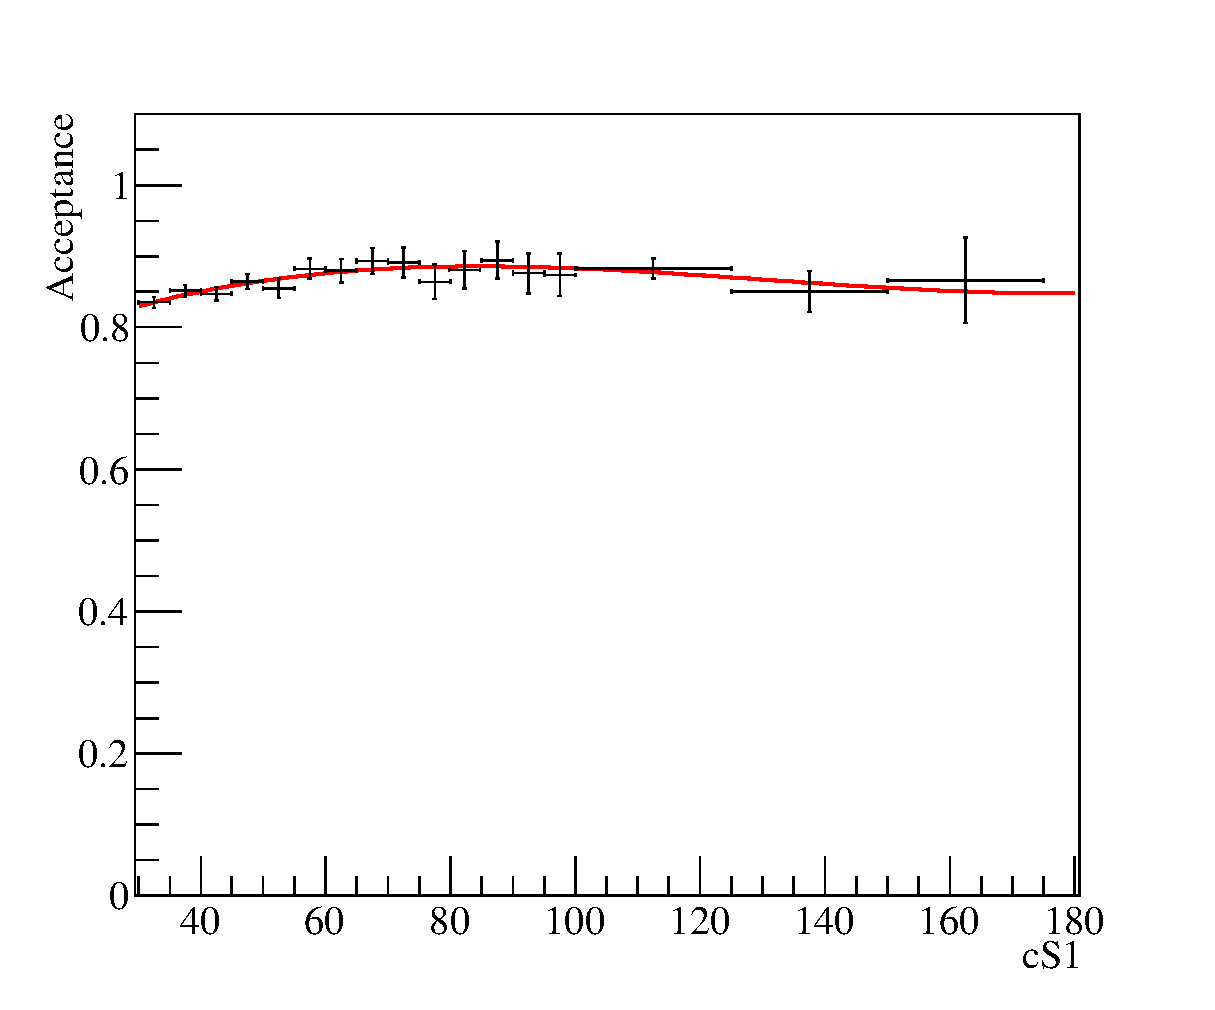
\includegraphics[width=1.\linewidth]{Figures/Acceptance.eps}}
\end{minipage}
\caption{The total acceptance of all cuts used, data from calibration in black and the fit in red.}
\label{fig:Acc}
\end{figure}

In order to estimate the energy deposition in this region we use the \Leff\ based method which is given in Eq.~\ref{eq:LeffEnergyScale}
\begin{equation}
\label{eq:LeffEnergyScale}
	E_{nr} = \frac{cS1}{L_y} \frac{1}{L_{eff}(E_{nr})} \frac{S_{ee}}{S_{nr}}
\end{equation}
The energy range in this region is bounded by the statistics of NR calibration data, namely $^{241}AmBe$.

The signal model is then produced by taking the event rate spectra converting it to S1, applying the acceptance and the detector response (explained in ~\cite{xe100_ana2012}) to give the expected event rate in the detector for each operator. In fig~\ref{fig:signal} is an example of ...

We divide our signal region into two bands in log(S2/S1). The bands are constructed such that the NR data sample is equally distributed between them. Each band is divided into several bins, for bins definitions see table (add table here and ref to figure). The number of bins is optimized using MC studies.

In order to estimate the background, we choose a control region in which we expect no signal. The control region we chose is from the ER band mean and above to include most of the background see fig.~\ref{fig:controlRegion}.

Discussion on Uncertainty for HighE, few words about crosschecks, and table summarizing uncertainties.

\begin{figure}[h!]
\begin{minipage}{1.\linewidth}
\centerline{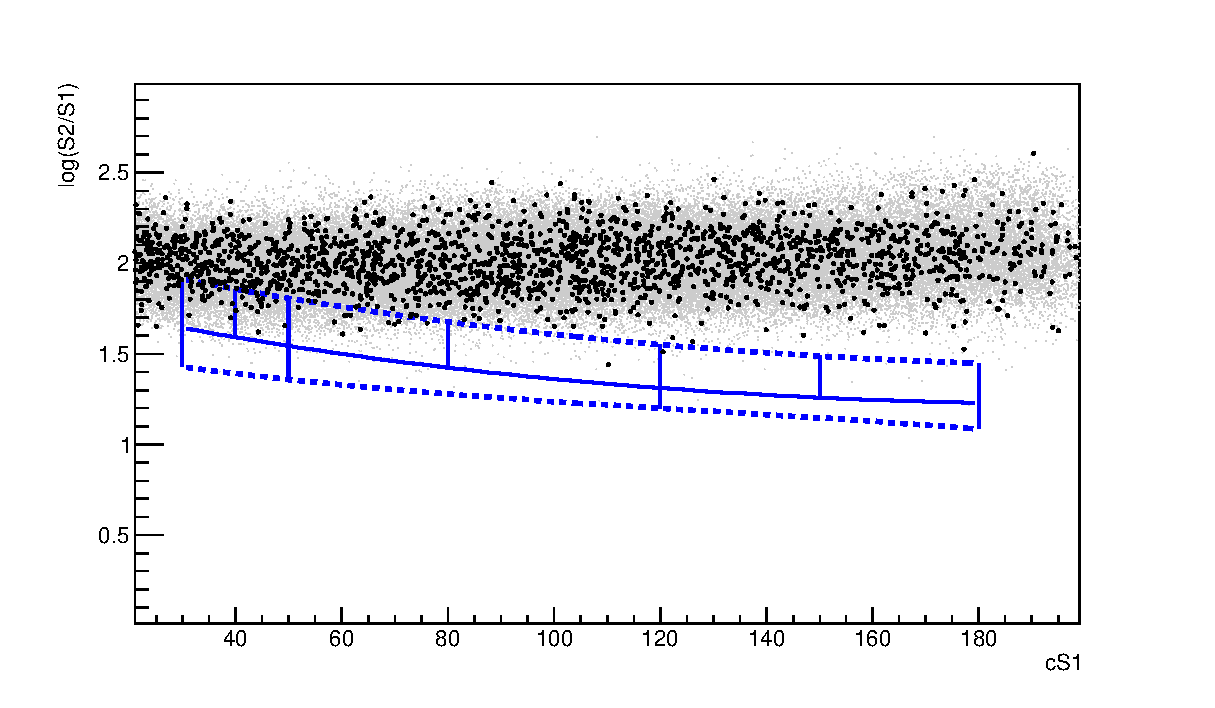
\includegraphics[width=1.\linewidth]{Figures/phasespace.eps}}
\end{minipage}
\caption{.}
\label{fig:Acc}
\end{figure}  


\subsubsection{Low Energy}
explain shortly the 2D signal model, and give ref to run combination paper.
explain shortly bck model and give ref to run combination paper. Discussion with table
summarizing uncertainties.


\subsection{Statistical Method}
Explanation of the likelihood methods used, short explaination of the likelihood parts and constraints for combination, joint usage of nuisance parameters {Leff}.
%\subsubsection{High Energy}
%likelihood function + uncertainties 
%\subsubsection{Low Energy}
%ref to run combination.


\section{Results}

limits on all operators. (including cdms comparison.)

\section{Summary}
\section{Acknowledgment}


%%% BIBLIOGRAPHY %%%

\bibliographystyle{apsrev}
\bibliography{EFTPaperBib}

\end{document}
